\documentclass[a4paper, 11pt]{article}

\usepackage[english]{babel}
\usepackage[utf8]{inputenc}
\usepackage[T1]{fontenc}
\usepackage{graphicx}
\usepackage{color}
\usepackage{amsmath,amssymb}
\usepackage{rotating} 
\usepackage{layaureo}
\usepackage{booktabs}
\usepackage{varioref}
%\usepackage{subfigure}
\usepackage{listings}
\usepackage{wrapfig}
\usepackage{siunitx}
\usepackage{physics}
\usepackage{subcaption} 
\usepackage{subfloat}
\usepackage{caption}
\usepackage{gensymb}

\sisetup{output-decimal-marker={.}}

\author{Jakub Skowronski & Alessandro Compagnucci}
\title{PROTO Trace}

\begin{document}


\maketitle

\section{Introduction}
 \paragraph{}
PROVA 

We are using a silicon detector of $200$ $\mu$$m$ thickness, which completely stops the incoming low energy charged particles ($\alpha$ or $p$) inside it. These charged particles cannot come out of the detector and this will be an issue to plot $\Delta$E-E graph, which is used to identify the incoming charged particle. For the particles stopping in the thin silicon detectors, it is foreseen to employ pulse shape discrimination techniques to discriminate between them. It is thus critical to preserve the shape of the original signal, in particular considering that the distance between the reaction chamber and the readout electronic is approximately 10m. For this reason, a second stage of signal treatment was added in the electronic chain between the pre-amplifiers and the readout which transform the signal from single-ended to differential module. Instead if we use the single ended amplifier the signal gets integrated over the entire length of the cable and information regarding the shape of the signal is lost and hence we will not be able to exactly identify the incoming charged particle.
         
These voltage signals can be analyzed offline. These signals carry the information on energy of the incoming particle and type of incoming particle.  To understand the type of the incoming particle we need to do the pulse shape analysis i.e. the rise time, fall time will be different for different types of incoming particles. But the exact information on the energy of the incoming particle is given by the height of the signal.The peak of these signals carry the information about the charge collected from the detector which is proportional to the energy of the incoming particles.
 

\paragraph{}
In the  second section of this report , the setup used to investigate the linearity of the electronic chain with respect to the amplitude of the input signal is described. In the third section, the characterization of the detectors with an alpha source is presented.In the second and third section results are also discussed,which basically emphasizes that the setup we are using is linear with respect to the energy incident on the detector and linearity is retained throughout the setup. The excellent energy resolution obtained and the linearity of the setup make it usable for spectroscopic studies. Moreover, the possibility to identify charged particles and light nuclei using pulse shape discrimination (for low energy particles) and/or E-$\Delta$E methods makes the setup versatile and of great interest for gamma spectroscopy.This setup when used in coincidence with the gamma detector it can reveal more information on the reaction dynamics and the decay of the nuclei produced in the reaction.


\section{Linearity of the Electronic Chain}
Checking the linear response of the electronic chain is an important step in any of the nuclear physics experiment. If we basically look at the experimental apparatus we are using we realize that in order to get the exact information about the energy of the incident particle, the response of each and every electronic device which we are using should behave linearly with respect to the energy of the incident particle. So in order to verify the above statement we constructed the chain as shown below and checked it.

\begin{figure}[h]
    \centering
    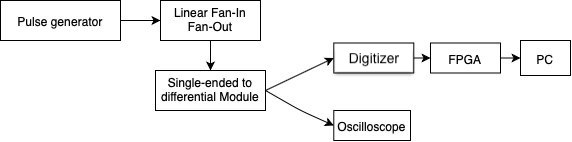
\includegraphics[scale = 0.5]{img/electronic_chain_diagram}
    \caption{Electronic chain}
    \label{fig:my_label}
\end{figure}


As in the above diagram pulse generator from the Berkeley nucleonics had to be connected to a linear Fan in Fan out module which basically reproduces the same pulse in 12 different ports. These 12 signals from Fan-in Fan-out circuit had to be connected to the Single-ended to differential module. In order to do so we made the cables for the 12 outputs from Fan-in Fan-out module by soldering and we connected it. The output of the differential amplifier is as shown in the following picture:


\begin{figure}[h]
 
\begin{subfigure}{0.5\textwidth}
%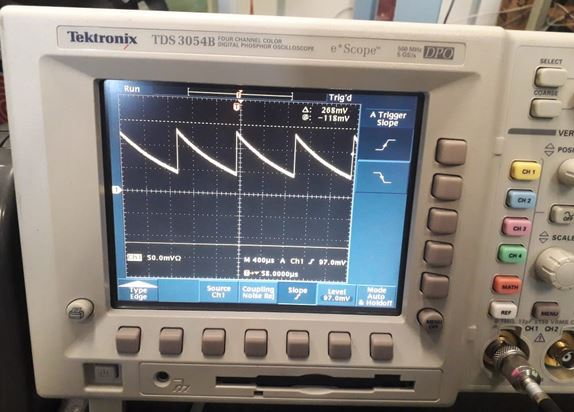
\includegraphics[width=0.9\linewidth, height=5cm]{test_signal_oscilloscope.JPG} 
\caption{output as seen in oscilloscope}
\label{fig:subim1}
\end{subfigure}
\begin{subfigure}{0.5\textwidth}
%\includegraphics[width=0.9\linewidth, height=5cm]{test_signal_pc.JPG}
\caption{output as seen in pc}
\label{fig:subim2}
\end{subfigure}
 
\caption{Input pulse characteristics $a)$ $Wave-form$ $:$ $Square-wave$ \newline $b)$ $Amplitude$ $:$ $0.2V$ and $c)$ $Fall-time$ $:$ $1ms$}
\label{fig:image2}
\end{figure}

         
         
         
\end{document}
